% ML-Driven PVT Variation Aware Leakage Estimation -- Digital VLSI Design course project report (Team 26)
% Tables in tables/*.tex are GENERATED from the result files by scripts/11_build_report_tables.py -- do not edit them by hand.
% Build (from this directory):  latexmk -pdf report.tex   (or: pdflatex report.tex, twice)
\documentclass[11pt,a4paper]{article}
\usepackage[margin=2.2cm]{geometry}
\usepackage[T1]{fontenc}
\usepackage[utf8]{inputenc}
\usepackage{lmodern}
\usepackage{microtype}
\usepackage{booktabs}
\usepackage{graphicx}
\usepackage{float}
\usepackage{amsmath,amssymb}
\usepackage{xcolor}
\usepackage{caption}
\usepackage{subcaption}
\usepackage{enumitem}
\usepackage{array}
\usepackage{adjustbox}
\usepackage{fancyhdr}
\usepackage[hidelinks]{hyperref}
\usepackage[capitalise,noabbrev]{cleveref}

\graphicspath{{../results/data_check/}{../results/models/}{../results/gates/}{../results/circuit/}}
\captionsetup{font=small,labelfont=bf}
\setlist{nosep}
\setlength{\parindent}{0pt}
\renewcommand{\arraystretch}{1.08}
\setlength{\emergencystretch}{3em}

\newcommand{\Vdd}{V_{DD}}
\newcommand{\Lmin}{L_{\min}}
\newcommand{\Weff}{W_{\mathrm{eff}}}
\newcommand{\Ifl}{I_{0}}

% ---- team (roll numbers of the other members to be filled in) ----
\newcommand{\RollManas}{XXXXXXXXXX}
\newcommand{\RollSoham}{XXXXXXXXXX}
\newcommand{\RollRithvik}{XXXXXXXXXX}
\newcommand{\RollGautam}{2023102059}

\pagestyle{fancy}
\fancyhf{}
\lhead{\small ML-Driven PVT Variation Aware Leakage Estimation}
\rhead{\small Team 26 -- Return of LUZAAZ}
\cfoot{\thepage}

\begin{document}

\begin{titlepage}
\centering
\vspace*{1.5cm}
{\large Digital VLSI Design --- Course Project\par}
\vspace{1.2cm}
{\LARGE\bfseries ML-Driven PVT Variation Aware\\[0.3em] Leakage Estimation\par}
\vspace{0.8cm}
{\large Machine-learning transistor models for the leakage of CMOS gates\\ and an 8-bit parity checker under process, voltage and temperature variation\par}
\vspace{1.6cm}
{\Large\bfseries Team 26 --- Return of LUZAAZ\par}
\vspace{0.8cm}
\begin{tabular}{ll}
\toprule
Name & Roll number\\
\midrule
Manas Inamdar & \RollManas\\
Soham Jahagirdar & \RollSoham\\
Sai Rithvik Achutuni & \RollRithvik\\
Gautam Gandhi & \RollGautam\\
\bottomrule
\end{tabular}
\vspace{1.4cm}

\begin{tabular}{ll}
Model file & PTM \texttt{22nm\_LP} (BSIM4)\\
Nominal supply & $\Vdd = 1\,\mathrm{V}$\\
Test circuit & 8-bit parity checker\\
Simulator & ngspice-47
\end{tabular}
\vfill
\begin{minipage}{0.86\textwidth}
\small\textbf{Summary.}
Four transistor models (NMOS/PMOS, ON/OFF), trained only on single-transistor SPICE data, predict the leakage of INV, NAND2, NOR2, AND2 and OR2
for all 18 input cases at 200 PVT corners with a \textbf{mean accuracy of 99.65\,\%} (median error 0.19\,\%), and the leakage of an 8-bit parity
checker built from 28 NAND2 gates for all 256 input vectors at the same corners with a \textbf{mean accuracy of 99.73\,\%} (median error 0.19\,\%).
The 99\,\% target is met at both levels.
\end{minipage}
\vspace{1cm}

{\large November 2026\par}
\end{titlepage}

\tableofcontents
\newpage
\setlength{\parskip}{0.35em}

\section{Introduction and setup}\label{sec:setup}

The static (leakage) current of a CMOS circuit depends strongly on process parameters, supply voltage and temperature (PVT). Estimating it with
full SPICE simulation for every corner and every input vector is expensive. This project replaces SPICE with machine learning in a hierarchical way:
\begin{enumerate}
  \item \textbf{Part A -- transistor models.} Single NMOS and PMOS transistors are simulated in their ON and OFF states over random PVT and bias
        conditions, and one ML model per case predicts the four terminal currents $(I_d, I_g, I_s, I_b)$.
  \item \textbf{Part B -- gates.} Using only these four models, the leakage of INV, NAND2, NOR2, AND2 and OR2 is predicted for every input combination
        (18 cases) at 200 random PVT corners and compared with transistor-level SPICE simulations of the gates.
  \item \textbf{Part C -- test circuit.} The leakage of the assigned test circuit is composed from the gate-level predictions and compared with a SPICE
        simulation of the complete netlist at the same corners.
\end{enumerate}

\subsection{Assignment and tools}
\begin{center}\small
\begin{tabular}{>{\bfseries}l p{0.62\textwidth}}
\toprule
Item & Value\\
\midrule
Team & 26 -- Return of LUZAAZ\\
Model file & PTM \texttt{22nm\_LP.pm} (low-power 22\,nm, BSIM4 \texttt{level=54}, \texttt{version=4.0}), NMOS and PMOS cards\\
Nominal supply & $\Vdd=1\,\mathrm{V}$, sampled uniformly in $0.9$--$1.1\,\mathrm{V}$\\
Channel length & $L=\Lmin=22\,\mathrm{nm}$; widths $W=1$--$8\times\Lmin$ for NMOS and PMOS\\
Test circuit & 8-bit parity checker\\
Simulator & ngspice-47 (official 64-bit Windows build, KLU solver), DC operating point (\texttt{op}) analyses in batch mode\\
Solver options & \texttt{.options gmin=1e-18 abstol=1e-18 reltol=1e-6 vntol=1e-9} in every netlist\\
Software & Python 3.12 with NumPy, pandas, scikit-learn, LightGBM and PyTorch; exact versions locked in \texttt{uv.lock}\\
Randomness & every random draw uses fixed seeds from \texttt{config/project.yaml} (base seed 20261105)\\
\bottomrule
\end{tabular}
\end{center}

Following a clarification in the course group, the drain and source junction areas are set to $AD=AS=W\cdot L_{\mathrm{diff}}$ with
$L_{\mathrm{diff}}=44\,\mathrm{nm}$ (the value used in the example netlist provided with the assignment) for every transistor in every netlist; perimeters (PD/PS) are not set.
The model-file header mentions $0.95\,\mathrm{V}$; the assigned $1\,\mathrm{V}$ is used throughout.

\subsection{Repository and pipeline}
All results in this report are produced by the numbered scripts in \texttt{scripts/}, run in order (Appendix~\ref{app:reproduce}), using the library
\texttt{src/dvdml/}. The scripts read every assignment parameter from \texttt{config/project.yaml} and the model card from \texttt{22nm\_LP.pm}.
Every table in this report is generated from the result files by \texttt{scripts/11\_build\_report\_tables.py}; no number in a table is typed by hand.
The location of each deliverable is listed in Appendix~\ref{app:deliverables}.

\section{Data generation}\label{sec:data}

\subsection{Sampling}
For each of the four cases (NMOS ON, NMOS OFF, PMOS ON, PMOS OFF), 10{,}000 samples were drawn. Every parameter is drawn independently;
$\Vdd$ is drawn first because the ranges of $V_d$ and $V_s$ depend on it (\cref{tab:sampling}). The five process parameters are drawn as the nominal
value of the model card multiplied by a factor uniform in $[0.9, 1.1]$, separately for NMOS and PMOS (so the PMOS threshold stays negative).
Gate and body voltages are fixed by the case.

\begin{table}[H]\centering\small
\begin{tabular}{ll}
\toprule
Parameter & Distribution\\
\midrule
$\Vdd$ & uniform, $1\,\mathrm{V}\pm10\,\%$\\
$V_d$, $V_s$ & uniform, $0$ to $\Vdd$\\
$W$ & uniform, $1\times\Lmin$ to $8\times\Lmin$ ($22$--$176\,\mathrm{nm}$)\\
Temperature & uniform, $-40$ to $125\,^\circ$C\\
\texttt{vth0}, \texttt{toxe}, \texttt{ndep}, \texttt{u0}, \texttt{xj} & uniform, nominal value of the card $\pm10\,\%$, separate NMOS/PMOS draws\\
$(V_g, V_b)$ & NMOS ON $(\Vdd,0)$, NMOS OFF $(0,0)$, PMOS ON $(0,\Vdd)$, PMOS OFF $(\Vdd,\Vdd)$\\
\bottomrule
\end{tabular}
\caption{Sampling distributions of the transistor datasets (assignment, Section 4).}\label{tab:sampling}
\end{table}

The random generator of each case is seeded with (base seed, case index, batch). A sample whose simulation fails would be replaced from a
deterministic extra batch so that every file has exactly 10{,}000 rows; no simulation failed. The four datasets
(\texttt{data/transistor/*.csv}, columns \texttt{vdd, temp, w, vd, vs, vg, vb, vth0, toxe, ndep, u0, xj, id, ig, is, ib}) took about two minutes
per case with parallel ngspice processes.

\subsection{Netlists}
Each sample is written as a self-contained single-transistor netlist (examples in \texttt{data/netlists/\allowbreak single\_transistor/}):
\begin{itemize}
  \item both model cards are inlined; the five sampled process values replace the nominal values in the card of the device under test;
  \item one MOSFET with $L=22\,\mathrm{nm}$, the sampled $W$ and $AD=AS=W\cdot L_{\mathrm{diff}}$;
  \item \textbf{one DC voltage source per terminal} ($V_d$, $V_g$, $V_s$, $V_b$), the sampled temperature (\texttt{.temp}) and the mandated
        \texttt{.options} line;
  \item an operating-point analysis that prints the four source currents with ten significant digits.
\end{itemize}
The terminal currents are the negated source currents, i.e.\ they are defined positive \emph{into} the device, so that $I_d+I_g+I_s+I_b=0$.

\subsection{Training, validation and test split}
Each 10{,}000-row dataset is split at random into 70\,\% training, 15\,\% validation and 15\,\% test rows (7{,}000 / 1{,}500 / 1{,}500) with a fixed
seed (\texttt{scripts/03\_make\_splits.py}, \texttt{data/splits/}). Model types, hyper-parameters and all design choices were selected on the validation
rows only; the test rows were used once, to report the final models.

\paragraph{Additional training data.} The assignment allows the number of samples to be increased. Two training-only sets were generated in the same way
(scripts \texttt{01b}, \texttt{01c}); the delivered 10{,}000-row datasets and the validation and test splits are unchanged:
\begin{itemize}
  \item \textbf{30{,}000 extra uniform rows per case} (\texttt{data/transistor\_extra/}), drawn from exactly the distributions of \cref{tab:sampling}.
        Rows 0--24{,}999 are added to the training set; rows 25{,}000--29{,}999 are a hold-out set that is never trained on.
  \item \textbf{20{,}000 rail-corner rows per case} (\texttt{data/transistor\_edge/}). $\Vdd$, temperature and process are drawn as above, but each of
        $V_d$ and $V_s$ is placed exactly at a rail (0 or $\Vdd$) with probability 40\,\%, within $0.1\,\Vdd\,u^2$ of a rail with probability 40\,\%
        and uniformly otherwise, and $W$ is drawn log-uniformly. In a logic gate every source and drain sits at, or within microvolts of, a rail,
        where uniform sampling places very few points. Only this a-priori fact is used---no gate or circuit SPICE result. Rows 0--15{,}999 are
        training rows, 16{,}000--17{,}999 join the validation set and 18{,}000--19{,}999 are a rail-corner hold-out.
\end{itemize}
In total 120{,}000 transistor simulations were run; none failed.

\subsection{Data check}
\paragraph{Kirchhoff check.} \Cref{tab:kirchhoff} gives the residual $|I_d+I_g+I_s+I_b|$ of every sample. For NMOS ON, NMOS OFF and PMOS ON the median
relative residual is about $10^{-10}$, i.e.\ the netlists conserve current to the printed precision. The larger \emph{relative} residuals---the PMOS
OFF case and the tail of NMOS ON---occur in samples whose currents are themselves at the numerical floor (29\,\% of the PMOS OFF rows have no current
above $10^{-16}$\,A); the \emph{absolute} residual never exceeds $5\times10^{-14}$\,A and is below $2\times10^{-15}$\,A for both OFF cases.
\begin{table}[H]
\centering
{\small
\begin{adjustbox}{max width=\linewidth}
\begin{tabular}{lrrrrr}
\toprule
case & abs. median [A] & abs. P95 [A] & abs. max [A] & rel. median & rel. P95 \\
\midrule
NMOS ON & $2.72\times10^{-16}$ & $4.12\times10^{-15}$ & $5.14\times10^{-14}$ & $2.55\times10^{-10}$ & $2.31\times10^{-4}$ \\
NMOS OFF & $1.76\times10^{-25}$ & $2.51\times10^{-22}$ & $5.39\times10^{-21}$ & $5.68\times10^{-11}$ & $2.62\times10^{-10}$ \\
PMOS ON & $6.84\times10^{-17}$ & $3.55\times10^{-15}$ & $4.43\times10^{-14}$ & $1.84\times10^{-10}$ & $8.73\times10^{-5}$ \\
PMOS OFF & $3.30\times10^{-17}$ & $3.19\times10^{-16}$ & $1.80\times10^{-15}$ & $1.19\times10^{-3}$ & $9.34\times10^{-1}$ \\
\bottomrule
\end{tabular}
\end{adjustbox}
}
\caption{Kirchhoff check on the four 10{,}000-row datasets: residual $|I_d+I_g+I_s+I_b|$ per sample, absolute and relative to the largest terminal current of the sample (relative values for samples whose largest current exceeds $10^{-16}$\,A).}
\label{tab:kirchhoff}
\end{table}



\paragraph{Numerical noise floor.} The current distributions (\cref{fig:dist}) show that not every value is physical signal. The gate current of
the OFF devices, for example, is never above $10^{-15}$\,A and otherwise takes a few discrete values that are multiples of a double-precision
rounding step; tighter solver tolerances reproduce the same values. Currents below $\Ifl=10^{-15}$\,A are therefore treated as the noise floor of
the reference: they cannot be learned and are not scored (\cref{sec:metrics}).

\begin{figure}[!htbp]\centering
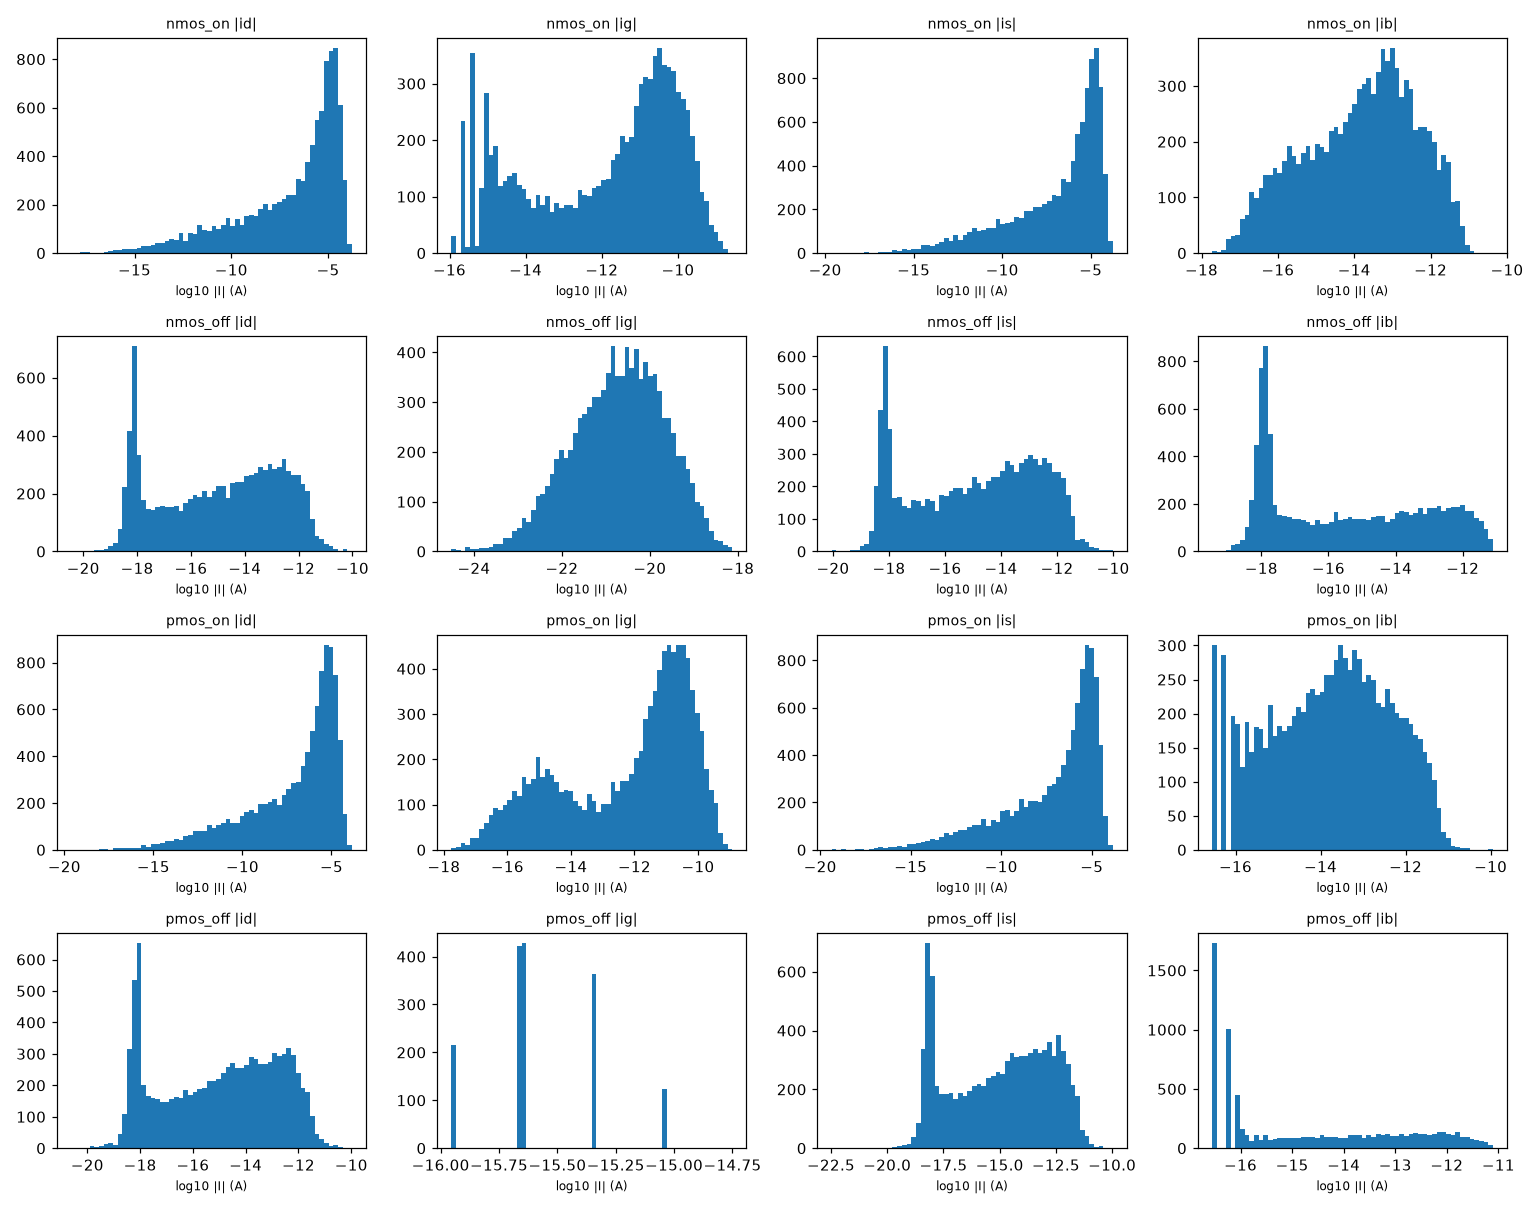
\includegraphics[width=0.95\textwidth]{distributions.png}
\caption{Magnitude distributions of the four terminal currents for the four cases (10{,}000 rows each).}\label{fig:dist}
\end{figure}

\paragraph{Trend plots.} \Cref{fig:trends} shows the three required trends. They come from controlled one-at-a-time SPICE sweeps (all other inputs at
nominal) built with the same netlist generator. All three follow the physically expected direction (\cref{tab:trends}): the OFF current grows by a
factor of about 400 from $-40$ to $125\,^\circ$C (sub-threshold conduction), falls by a factor of 35--46 when $|V_{th0}|$ rises from $-10\,\%$ to
$+10\,\%$, and the gate (oxide-tunnelling) current of an ON device falls by a factor of about 30 when \texttt{toxe} grows from $-10\,\%$ to $+10\,\%$.
\begin{table}[H]
\centering
{\small
\begin{adjustbox}{max width=\linewidth}
\begin{tabular}{llrll}
\toprule
case & expected trend & ratio & sweep end points & check \\
\midrule
NMOS OFF & OFF $I_d$ increases with temperature & 415.3 & 125C / -40C & pass \\
PMOS OFF & OFF $I_d$ increases with temperature & 389.4 & 125C / -40C & pass \\
NMOS OFF & OFF $I_d$ decreases as vth0 increases & 45.61 & |vth0| -10\% / +10\% & pass \\
PMOS OFF & OFF $I_d$ decreases as vth0 increases & 34.82 & |vth0| -10\% / +10\% & pass \\
NMOS ON & ON $I_g$ decreases as toxe increases & 29.57 & toxe -10\% / +10\% & pass \\
PMOS ON & ON $I_g$ decreases as toxe increases & 32.2 & toxe -10\% / +10\% & pass \\
\bottomrule
\end{tabular}
\end{adjustbox}
}
\caption{Automatic checks of the three trend sweeps: expected direction and ratio of the currents at the two ends of each sweep (all other inputs fixed at nominal).}
\label{tab:trends}
\end{table}



\begin{figure}[!htbp]\centering
\begin{subfigure}{0.49\textwidth}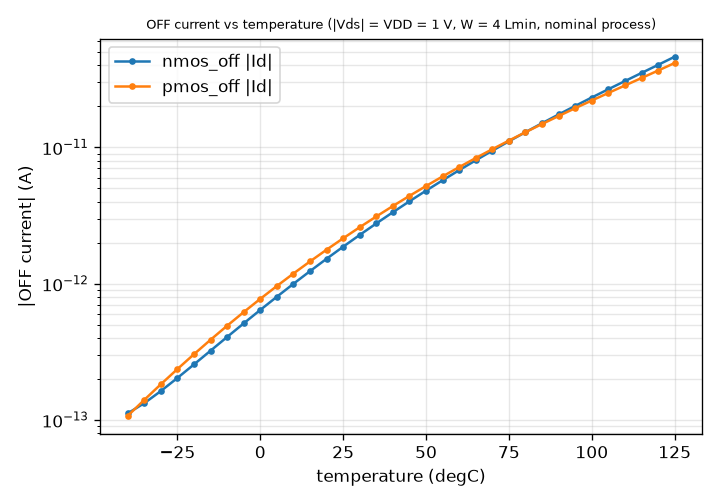
\includegraphics[width=\linewidth]{trend_off_vs_temperature.png}\caption{OFF current vs temperature}\end{subfigure}
\begin{subfigure}{0.49\textwidth}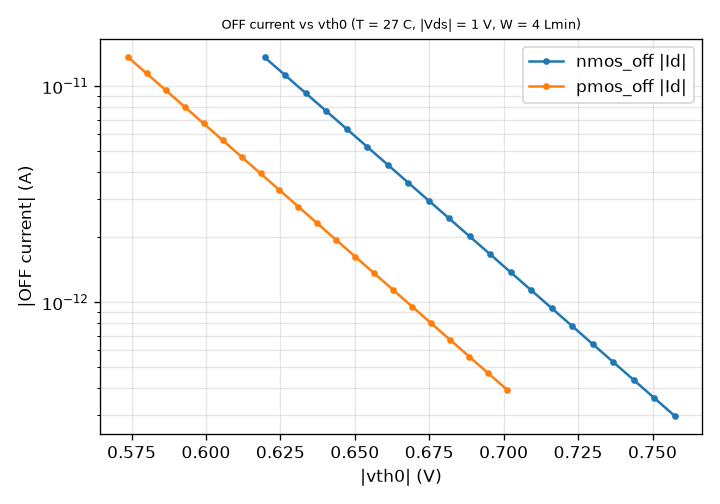
\includegraphics[width=\linewidth]{trend_off_vs_vth0.png}\caption{OFF current vs vth0}\end{subfigure}\\[0.4em]
\begin{subfigure}{0.49\textwidth}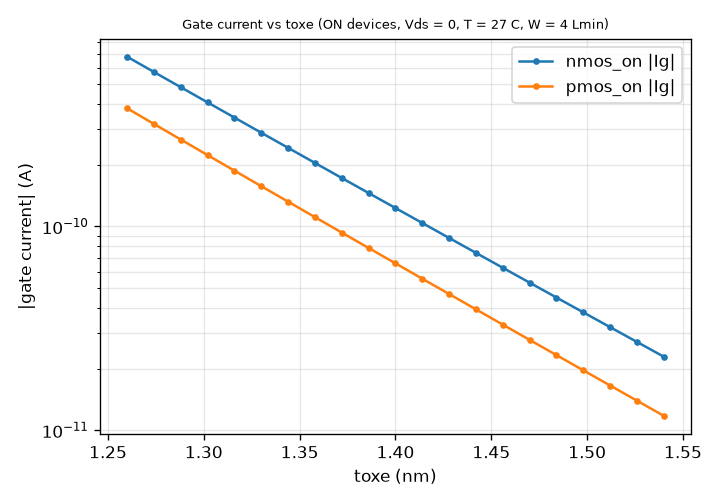
\includegraphics[width=\linewidth]{trend_ig_vs_toxe.png}\caption{Gate current vs toxe (ON devices)}\end{subfigure}
\caption{The three trend plots of the data check.}\label{fig:trends}
\end{figure}

\section{Transistor models}\label{sec:models}

\subsection{Targets, inputs and metrics}\label{sec:metrics}
The terminal currents span about ten decades ($10^{-15}$ to $10^{-4}$\,A), $I_d$ and $I_s$ change sign, and part of the data is numerical noise
(\cref{sec:data}). The models therefore never predict $I$ directly:
\begin{itemize}
  \item \textbf{Signed-log target} for currents that change sign: $y=\operatorname{asinh}(I/\Ifl)/\ln 10$ with $\Ifl=10^{-15}$\,A. It behaves like
        $\operatorname{sign}(I)\log_{10}(2|I|/\Ifl)$ for $|I|\gg\Ifl$, is linear and exactly zero at $I=0$, and so handles signs, zeros and ten decades
        in one continuous variable.
  \item \textbf{Log target} $y=\log_{10}|I|$ for currents that never change sign (gate current of ON devices, body currents), trained on the rows
        above the floor; the sign is constant and stored with the model.
  \item \textbf{Inputs}: 15 physics-motivated features---$\log_{10}W$, $1000/T$, $\Vdd$, $V_d$, $V_s$, $V_{ds}$, $V_{gs}$, $V_{gd}$, $V_{bs}$, $V_{bd}$,
        $|V_{th0}|$, \texttt{toxe}, $\log_{10}$\texttt{ndep}, \texttt{u0}, \texttt{xj}---standardised to zero mean and unit variance.
\end{itemize}
\textbf{Metrics.} The relative error $(I_{ML}-I_{SPICE})/|I_{SPICE}|$ is evaluated on \emph{resolved} samples, $|I_{SPICE}|>\Ifl$; below the floor
the reference itself is noise. We report the median and the 95th percentile (P95) of its absolute value and its mean (bias). Currents with fewer
than 5\,\% resolved samples (the gate current of OFF devices, which is \emph{never} resolved) are not scored. $R^2$ is computed on the signed-log
target, because on a linear scale it would be dominated by the largest ON currents.

\subsection{Model comparison}\label{sec:comparison}
Four model types were trained and compared for every case (\texttt{scripts/04\_compare\_models.py}). Each predicts the signed log of all four
currents from the 15 features and is trained on the 7{,}000 training rows; every hyper-parameter setting was scored on the validation rows with
score $=\frac12(\text{median}+\text{P95})$ of the relative error, macro-averaged over the scored currents (64 trials in total).
\begin{enumerate}
  \item \textbf{Multi-layer perceptron (MLP)} in PyTorch: 3 hidden layers of 96 or 128 tanh units, float64, Adam (cosine learning-rate decay from
        $3\times10^{-3}$, 1200 epochs, best validation epoch kept), then full-batch L-BFGS polishing.
  \item \textbf{Gradient-boosted trees} (LightGBM): one booster per current, 31 or 127 leaves, learning rate 0.05, early stopping on validation.
  \item \textbf{Kernel ridge regression} with an RBF kernel, $\gamma\in\{0.01,0.03,0.1\}$, $\alpha\in\{10^{-5},10^{-3}\}$.
  \item \textbf{Polynomial ridge regression}, degree 3 or 4, $\alpha\in\{10^{-3},10^{-1},10\}$.
\end{enumerate}
\begin{table}[H]
\centering
{\small
\begin{adjustbox}{max width=\linewidth}
\begin{tabular}{llrrrrl}
\toprule
case & model type & R2 & median err & P95 err & score & best hyper-parameters \\
\midrule
NMOS ON & MLP & 0.9963 & 4.30\% & 22.29\% & 0.1329 & 3 hidden layers x 128 tanh units \\
NMOS ON & LightGBM & 0.9976 & 12.63\% & 61.72\% & 0.3718 & leaves: 31 \\
NMOS ON & Kernel ridge & 0.9281 & 69.44\% & 5359.93\% & 27.15 & gamma: 0.01, alpha: 0.001 \\
NMOS ON & Polynomial ridge & 0.9068 & 71.43\% & 30690.41\% & 153.8 & degree: 4, alpha: 10.0 \\
NMOS OFF & MLP & 0.9951 & 1.69\% & 14.82\% & 0.08256 & 3 hidden layers x 96 tanh units \\
NMOS OFF & LightGBM & 0.9794 & 8.78\% & 63.18\% & 0.3598 & leaves: 31 \\
NMOS OFF & Kernel ridge & 0.9316 & 42.69\% & 161.28\% & 1.02 & gamma: 0.01, alpha: 0.001 \\
NMOS OFF & Polynomial ridge & 0.9302 & 41.67\% & 232.97\% & 1.373 & degree: 4, alpha: 0.1 \\
PMOS ON & MLP & 0.9995 & 2.04\% & 12.16\% & 0.07098 & 3 hidden layers x 96 tanh units \\
PMOS ON & LightGBM & 0.9968 & 13.15\% & 65.96\% & 0.3955 & leaves: 31 \\
PMOS ON & Kernel ridge & 0.9327 & 68.42\% & 4639.72\% & 23.54 & gamma: 0.01, alpha: 0.001 \\
PMOS ON & Polynomial ridge & 0.9137 & 70.11\% & 27706.76\% & 138.9 & degree: 4, alpha: 10.0 \\
PMOS OFF & MLP & 0.995 & 4.29\% & 24.75\% & 0.1452 & 3 hidden layers x 128 tanh units \\
PMOS OFF & LightGBM & 0.9785 & 8.56\% & 65.10\% & 0.3683 & leaves: 31 \\
PMOS OFF & Kernel ridge & 0.9383 & 35.69\% & 151.66\% & 0.9368 & gamma: 0.03, alpha: 0.001 \\
PMOS OFF & Polynomial ridge & 0.9287 & 40.06\% & 187.49\% & 1.138 & degree: 4, alpha: 0.001 \\
\bottomrule
\end{tabular}
\end{adjustbox}
}
\caption{Model comparison on the \emph{validation} set: 4 model types $\times$ 4 cases (best hyper-parameters of each type). $R^2$ on the signed-log target; relative errors on resolved currents ($|I|>10^{-15}$\,A), averaged over the scored currents; score $=\frac12$(median + P95), lower is better. Sorted by score within each case.}
\label{tab:comparison}
\end{table}



\textbf{The MLP is the best model type in all four cases}, with a score 2.5--5 times lower than the runner-up (LightGBM). Kernel ridge and polynomial
ridge assume a smooth global dependence and cannot follow exponential, threshold-like currents over ten decades; their P95 errors reach hundreds to
tens of thousands of percent. Gradient boosting is robust but piecewise constant and cannot reach the precision of the MLP. $R^2$ alone is misleading
here: LightGBM has the higher $R^2$ for NMOS ON, yet a three times larger median error. The MLP was therefore selected for all four cases.

\subsection{From the comparison winner to the final models}\label{sec:final_models}
With the comparison winner (one 4-output MLP per case, trained on 7{,}000 rows) the gate-level mean accuracy was 92.8\,\% (\cref{tab:stages}),
below the target. An analysis of \emph{which} transistor currents determine gate leakage, carried out on transistor data and on the structure of
the gate-level composition (\cref{sec:gates_method}), identified three causes:
\begin{enumerate}
  \item \textbf{Only some currents matter.} The gate leakage is composed from the gate current of ON devices, the channel currents of OFF devices and
        the body currents; the channel current of ON devices is fixed by Kirchhoff's law and never taken from the model (\cref{sec:gates_method}).
        For this low-power card about 98\,\% of the gate leakage at nominal temperature is gate-oxide tunnelling of the ON devices, about 2\,\%
        sub-threshold conduction and about 0.1\,\% junction current. A shared 4-output network spends most of its capacity on ON $I_d/I_s$, which
        the composition does not use.
  \item \textbf{Gates operate at the corners of the input space.} In a gate every drain and source sits at a rail, i.e.\ at a corner of the uniformly
        sampled $(V_d,V_s)$ square, where the training data is sparse and the error of the 4-output model was 2--3 times its average.
  \item \textbf{Effective width.} BSIM4 scales channel and tunnelling currents with $\Weff=W-2\,w_{\mathrm{int}}$ ($w_{\mathrm{int}}=5\,\mathrm{nm}$ in
        both cards), which is only 55\,\% of $W$ at $W=\Lmin$---the width used by the gates.
\end{enumerate}
The final models keep the winning model type (tanh MLP, Adam + L-BFGS) and change how it is used (\texttt{src/dvdml/ml\_v2.py},
\texttt{scripts/05d\_train\_per\_current.py}):
\begin{itemize}
  \item \textbf{one network ensemble per terminal current} ($4$ cases $\times$ $4$ currents $=16$ networks in four model files);
  \item \textbf{width-normalised targets}, $I/(\Weff/\Lmin)$ for $I_d$, $I_g$, $I_s$ and $I/(W/\Lmin)$ for $I_b$ (junction area $\propto W$);
  \item \textbf{six additional physics features}: oxide fields $V_{gs}/t_{ox}$, $V_{gd}/t_{ox}$, $\Vdd/t_{ox}$, gate overdrives $|V_{gs}|-|V_{th0}|$,
        $|V_{gd}|-|V_{th0}|$, and $|V_{th0}|/kT$ (21 inputs in total);
  \item \textbf{training data}: the 7{,}000 training rows plus the 25{,}000 extra uniform rows, and for the currents that dominate leakage
        (ON $I_g$, OFF $I_d/I_s$) the 16{,}000 rail-corner rows (\cref{sec:data});
  \item a fixed sample weight $1+4\,(e(V_d)+e(V_s))$, $e(v)=\exp(-\text{distance to the nearer rail}/0.05\Vdd)$, that emphasises the rails;
  \item \textbf{network}: 4 hidden layers of 128 tanh units (about 52{,}000 weights), Adam in float32 (1500 epochs, batch 512, learning rate
        $3\times10^{-3}$ with cosine decay, best validation state kept), then up to six float64 L-BFGS rounds, each kept only if the validation loss improves;
  \item an \textbf{ensemble} of three networks with different seeds for the leakage-relevant currents (prediction = mean in target space).
\end{itemize}
The settings of the 16 networks are listed in \cref{tab:settings}. Every choice was made on transistor data (validation rows, the uniform hold-out and the
rail-corner hold-out); no gate or circuit SPICE value was used for training, calibration or model selection. \Cref{tab:stages} shows the effect of
the successive changes on the gate and circuit accuracy.
\begin{table}[H]
\centering
{\small
\begin{adjustbox}{max width=\linewidth}
\begin{tabular}{llrrrr}
\toprule
model stage & level & mean accuracy & median err & P95 err & max err \\
\midrule
one 4-output MLP per case, 7k rows & gate (3,600 runs) & 92.79\% & 5.53\% & 19.56\% & 59.36\% \\
one 4-output MLP per case, 7k rows & circuit (51,200 runs) & 92.49\% & 6.38\% & 19.12\% & 46.22\% \\
one MLP per current, I/(W/Lmin) target & gate (3,600 runs) & 96.57\% & 2.39\% & 9.10\% & 38.68\% \\
one MLP per current, I/(W/Lmin) target & circuit (51,200 runs) & 97.90\% & 1.85\% & 3.90\% & 22.78\% \\
+ effective-width target I/(W\_eff/Lmin) & gate (3,600 runs) & 97.63\% & 1.64\% & 5.86\% & 41.46\% \\
+ effective-width target I/(W\_eff/Lmin) & circuit (51,200 runs) & 97.78\% & 1.86\% & 4.85\% & 26.23\% \\
+ rail-corner training rows (final) & gate (3,600 runs) & 99.65\% & 0.19\% & 1.20\% & 5.68\% \\
+ rail-corner training rows (final) & circuit (51,200 runs) & 99.73\% & 0.19\% & 0.79\% & 1.63\% \\
\bottomrule
\end{tabular}
\end{adjustbox}
}
\caption{Gate- and circuit-level accuracy of the successive model stages (same SPICE references, same composition code).}
\label{tab:stages}
\end{table}


\begin{table}[H]
\centering
{\small
\begin{adjustbox}{max width=\linewidth}
\begin{tabular}{lllrll}
\toprule
case & current & target & members & rail-corner data & width normalisation \\
\midrule
NMOS ON & id & asinh (signed log) & 3 & yes & Weff \\
NMOS ON & ig & log10|I| & 3 & yes & Weff \\
NMOS ON & is & asinh (signed log) & 1 & no & Weff \\
NMOS ON & ib & log10|I| & 3 & no & W \\
NMOS OFF & id & asinh (signed log) & 3 & yes & Weff \\
NMOS OFF & ig & asinh (signed log) & 1 & no & W \\
NMOS OFF & is & asinh (signed log) & 3 & yes & Weff \\
NMOS OFF & ib & log10|I| & 3 & no & W \\
PMOS ON & id & asinh (signed log) & 1 & no & Weff \\
PMOS ON & ig & log10|I| & 3 & yes & Weff \\
PMOS ON & is & asinh (signed log) & 1 & no & Weff \\
PMOS ON & ib & log10|I| & 3 & no & W \\
PMOS OFF & id & asinh (signed log) & 3 & yes & Weff \\
PMOS OFF & ig & asinh (signed log) & 1 & no & W \\
PMOS OFF & is & asinh (signed log) & 3 & yes & Weff \\
PMOS OFF & ib & log10|I| & 3 & no & W \\
\bottomrule
\end{tabular}
\end{adjustbox}
}
\caption{Settings of the 16 per-current networks of the final models (all: 21 inputs, 4 hidden layers of 128 tanh units, Adam 1500 epochs + L-BFGS polish).}
\label{tab:settings}
\end{table}



\subsection{Final models on the test set}\label{sec:test}
\Cref{tab:chosen_macro,tab:chosen} report the final models on the 1{,}500 test rows of each case, evaluated once; \cref{fig:pvs} shows predicted
against SPICE currents. The four model files are \texttt{models/<case>.joblib}; their prediction is pure NumPy.
\begin{table}[H]
\centering
{\small
\begin{adjustbox}{max width=\linewidth}
\begin{tabular}{llrrr}
\toprule
case & currents scored & R2 & median err & P95 err \\
\midrule
NMOS ON & id,ig,is,ib & 0.9977 & 6.13\% & 25.41\% \\
NMOS OFF & id,is,ib & 0.9887 & 1.10\% & 6.63\% \\
PMOS ON & id,ig,is,ib & 0.9989 & 2.72\% & 11.31\% \\
PMOS OFF & id,is,ib & 0.9754 & 1.93\% & 10.42\% \\
\bottomrule
\end{tabular}
\end{adjustbox}
}
\caption{Final models on the \emph{test} set (1{,}500 rows per case, evaluated once): macro-average over the scored currents.}
\label{tab:chosen_macro}
\end{table}


\begin{table}[H]
\centering
{\small
\begin{adjustbox}{max width=\linewidth}
\begin{tabular}{llrrrrr}
\toprule
case & current & resolved & R2 & median err & P95 err & bias \\
\midrule
NMOS ON & id & 98.87\% & 0.9981 & 12.69\% & 99.77\% & 21.93\% \\
NMOS ON & ig & 82.20\% & 0.9952 & 0.59\% & 7.22\% & 0.04\% \\
NMOS ON & is & 98.87\% & 0.9978 & 14.69\% & 46.26\% & 7.08\% \\
NMOS ON & ib & 75.93\% & 0.9986 & 0.27\% & 1.63\% & 0.05\% \\
NMOS OFF & id & 53.33\% & 0.9992 & 1.88\% & 9.43\% & -0.02\% \\
NMOS OFF & ig & 0.00\% & -- & -- & -- & -- \\
NMOS OFF & is & 53.80\% & 0.9942 & 1.28\% & 9.59\% & -0.20\% \\
NMOS OFF & ib & 43.47\% & 0.9729 & 0.15\% & 0.86\% & -0.40\% \\
PMOS ON & id & 98.87\% & 0.9987 & 3.91\% & 14.07\% & -0.19\% \\
PMOS ON & ig & 85.20\% & 0.9992 & 0.16\% & 0.75\% & 0.02\% \\
PMOS ON & is & 98.87\% & 0.9994 & 6.47\% & 27.88\% & -1.69\% \\
PMOS ON & ib & 75.13\% & 0.9983 & 0.33\% & 2.55\% & -0.01\% \\
PMOS OFF & id & 54.13\% & 0.9969 & 2.64\% & 15.23\% & -1.38\% \\
PMOS OFF & ig & 0.00\% & -- & -- & -- & -- \\
PMOS OFF & is & 54.60\% & 0.9929 & 2.94\% & 13.80\% & 0.67\% \\
PMOS OFF & ib & 44.33\% & 0.9364 & 0.19\% & 2.23\% & -0.11\% \\
\bottomrule
\end{tabular}
\end{adjustbox}
}
\caption{Final models on the test set, per terminal current (errors on resolved samples, $|I|>10^{-15}$\,A; OFF-state $I_g$ is below the floor in every row and is not scored).}
\label{tab:chosen}
\end{table}



%RETRAIN-PARAGRAPH%

The currents that determine gate leakage are predicted very accurately. On the test rows the ON-state gate current has a median error of
0.2--0.6\,\% and the OFF-state channel currents 1.3--2.9\,\%. At the gate operating points themselves---rail-corner hold-out rows with $V_d$ and $V_s$
exactly at a rail, never used for training or selection---the ON gate current is within 0.07--0.25\,\% and the OFF channel currents within
1.0--2.3\,\% (median, \cref{tab:rails}). The body currents of the ON devices show large relative errors at the exact rails, because with
$V_{bs}=V_{bd}=0$ their junction currents are only just above the $10^{-15}$\,A floor; they contribute about 0.1\,\% of the gate leakage, so these
errors are irrelevant at gate level.
\begin{table}[H]
\centering
{\small
\begin{adjustbox}{max width=\linewidth}
\begin{tabular}{llrrrr}
\toprule
case & current & rows & median err & P95 err & bias \\
\midrule
NMOS ON & ig & 277 & 0.25\% & 1.64\% & -0.23\% \\
PMOS ON & ig & 235 & 0.07\% & 0.26\% & -0.02\% \\
NMOS OFF & id & 194 & 1.35\% & 5.13\% & 0.13\% \\
NMOS OFF & is & 195 & 0.99\% & 3.92\% & -0.20\% \\
PMOS OFF & id & 212 & 1.86\% & 7.51\% & 0.44\% \\
PMOS OFF & is & 212 & 2.29\% & 7.90\% & 0.85\% \\
NMOS ON & ib & 286 & 1.93\% & 49.96\% & -78.48\% \\
PMOS ON & ib & 248 & 1.84\% & 36.36\% & 16.39\% \\
\bottomrule
\end{tabular}
\end{adjustbox}
}
\caption{Error of the final models at the gate operating points: held-out rail-corner rows with $V_d$ and $V_s$ both exactly at $0$ or $V_{DD}$ (never used for training or selection), for the currents that enter the gate leakage.}
\label{tab:rails}
\end{table}



\begin{figure}[!htbp]\centering
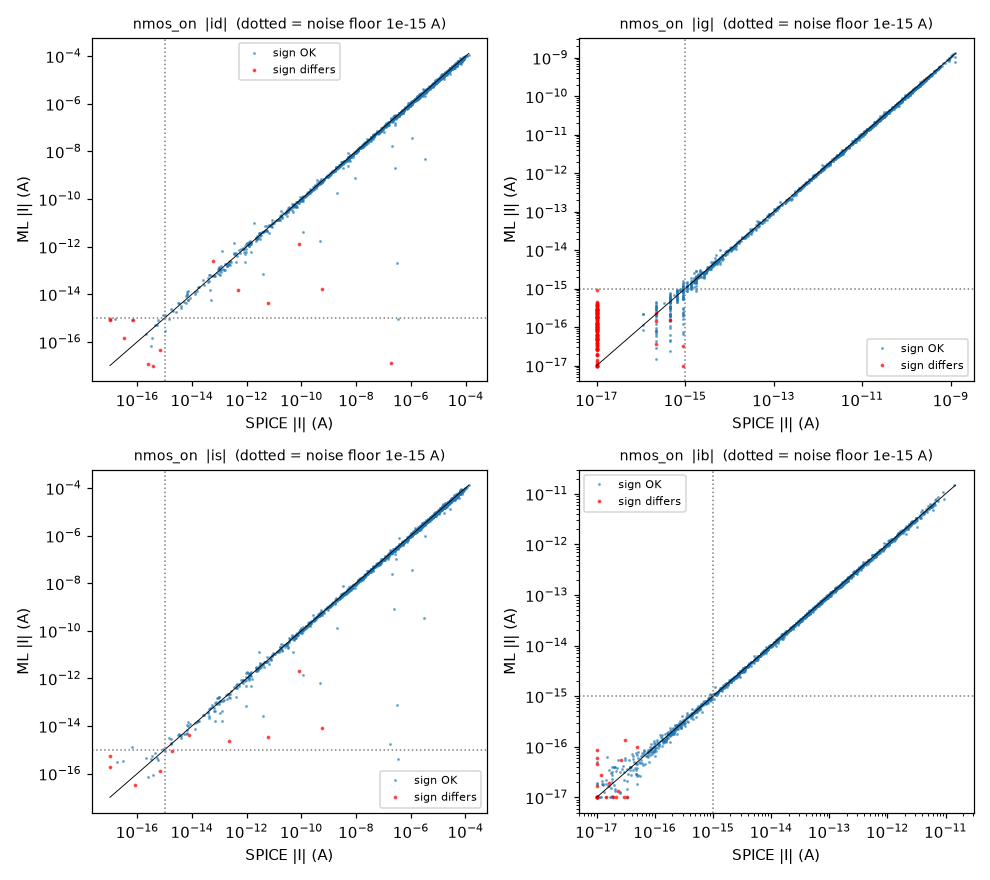
\includegraphics[width=.49\textwidth]{pred_vs_spice_nmos_on.png}\hfill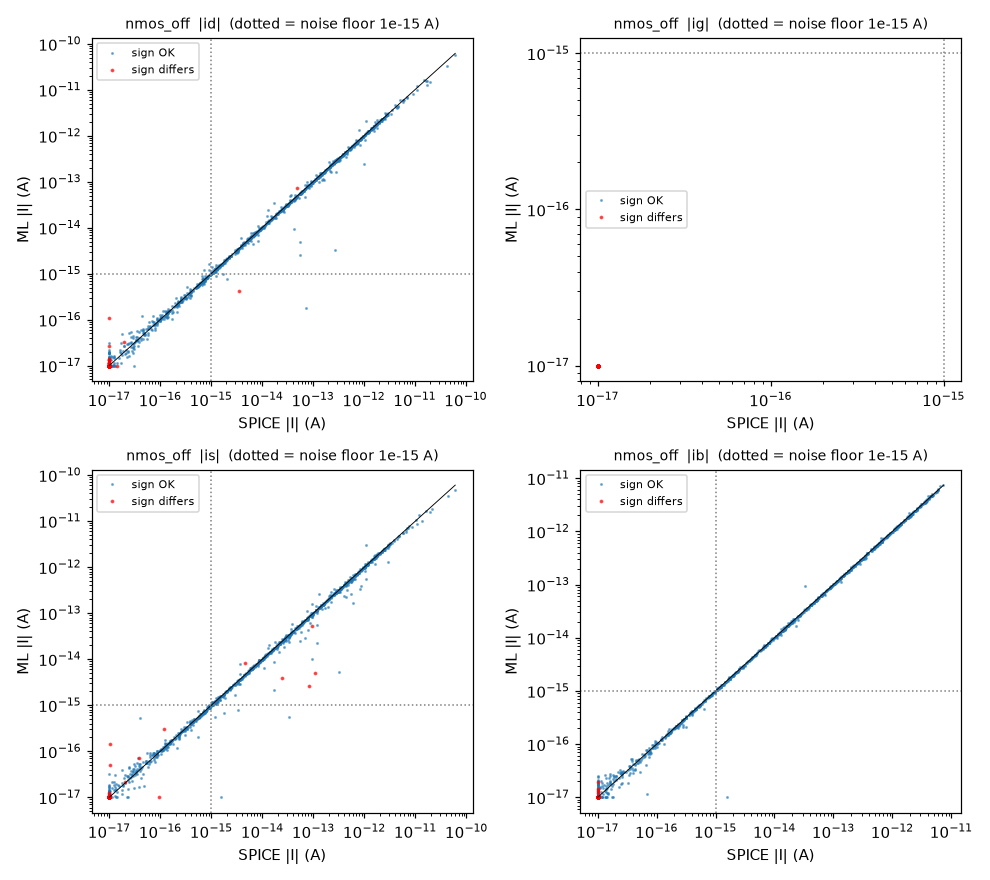
\includegraphics[width=.49\textwidth]{pred_vs_spice_nmos_off.png}\\[0.3em]
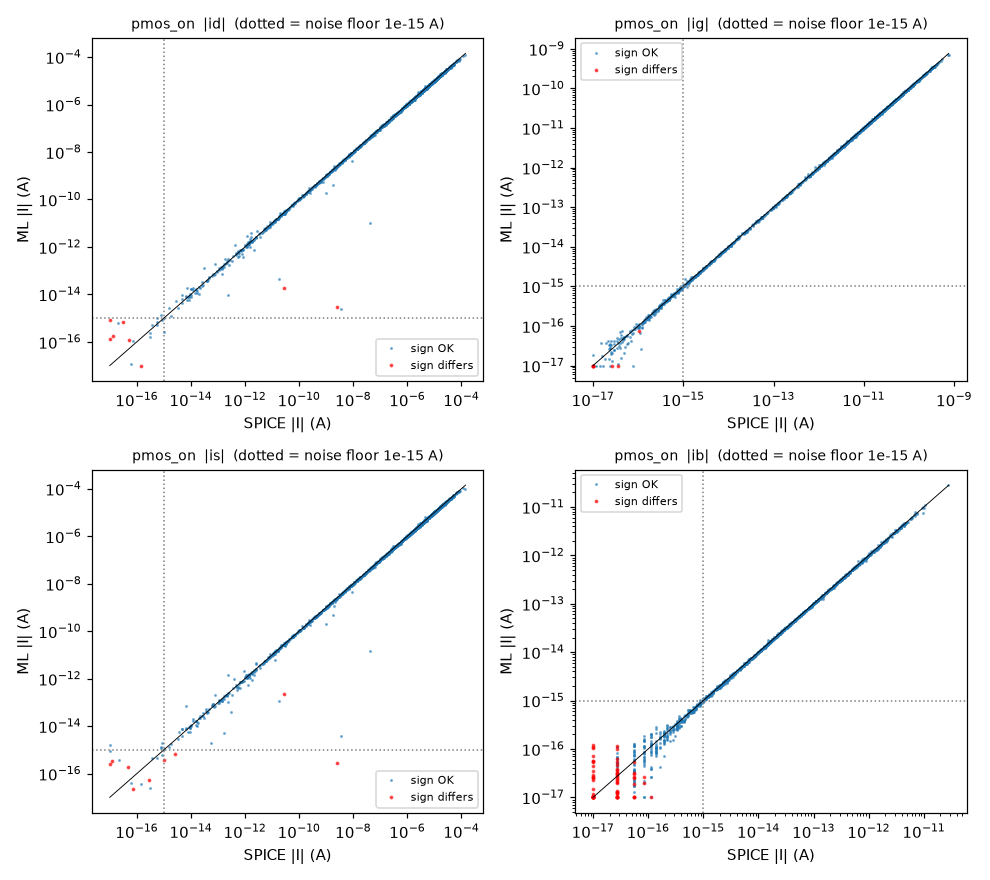
\includegraphics[width=.49\textwidth]{pred_vs_spice_pmos_on.png}\hfill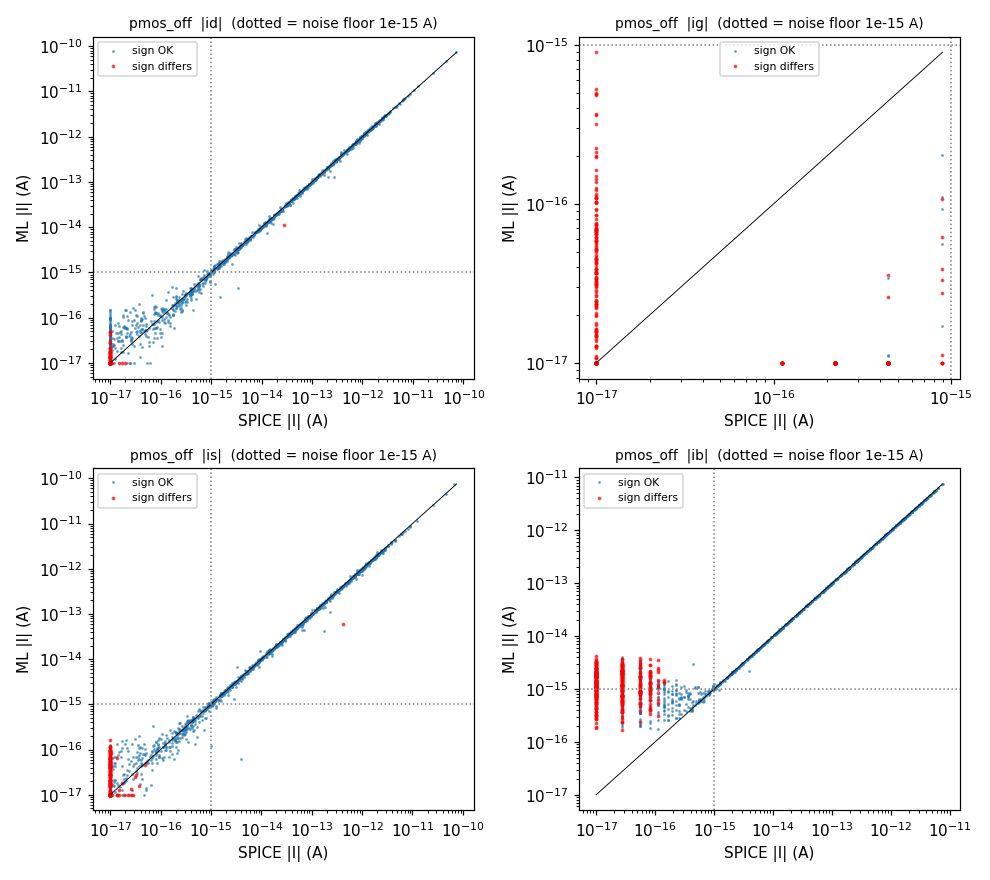
\includegraphics[width=.49\textwidth]{pred_vs_spice_pmos_off.png}
\caption{Predicted versus SPICE terminal currents on the test set for the four final models (absolute values, log axes).}\label{fig:pvs}
\end{figure}

\paragraph{Reason for the final choice.} The MLP was chosen because it was the most accurate model type in all four cases of the validation
comparison (\cref{tab:comparison}). It was then specialised per current, because the gate leakage depends on a few currents at the rail corners of the
input space, and a network devoted to each of these currents---with physically normalised targets and training data where gates operate---is both
more accurate there and still predicts all four terminal currents of every case, as required.

\section{Gate-level validation}\label{sec:gates}

\subsection{Gates, corners and SPICE reference}
The five gates are standard static CMOS circuits; AND2 is a NAND2 followed by an INV and OR2 a NOR2 followed by an INV, and both are simulated in
SPICE as complete gates. Transistor widths (in multiples of $\Lmin$) are INV $W_n=1$, $W_p=2$; NAND2 $W_n=W_p=2$; NOR2 $W_n=1$, $W_p=4$
(\cref{app:assumptions}). One table of gate topologies (\texttt{src/dvdml/gates.py}) generates both the SPICE netlists and the ML prediction,
so the two always describe the same circuit.

A \emph{corner} is one random draw of $\Vdd$, temperature and the five process parameters, from the distributions of \cref{tab:sampling}; all NMOS of
a gate share one process draw and all PMOS another. The same 200 corners (\texttt{data/gates/corners.csv}) are used for every gate and input
combination and again for the test circuit, giving $18\times200=3{,}600$ SPICE runs. Inputs are ideal sources at exactly $0$ or $\Vdd$; a 0\,V source
in the ground rail makes the return current measurable. Each run records the leakage, the output voltage and the internal node voltages ($x$ between the
series NMOS of NAND2, $y$ between the series PMOS of NOR2, and the NAND2/NOR2 output $n$ inside AND2/OR2). Example netlists are in \texttt{data/netlists/gates/}.

\paragraph{Leakage definition.} The leakage of a gate is the total static current delivered by all sources at $\Vdd$ (supply plus inputs held high).
By Kirchhoff's law it equals the current absorbed by the sources at $0$\,V; both are recorded and agree.

\paragraph{Validity of the reference.} With exactly the mandated solver options, ngspice converged to an invalid operating point in 59 of the 3{,}600
runs (for example an AND2 output stuck at $7\times10^{-5}$\,V instead of $4\times10^{-8}$\,V, which made the leakage 200 times too large) and did not
converge in 66 more. Every run was therefore solved twice: with exactly the mandated options, and with one additional options line that tightens the
tolerances ($\mathrm{abstol}=10^{-15}$, $\mathrm{reltol}=10^{-9}$, $\mathrm{vntol}=10^{-12}$). The mandated result is the reference whenever the two agree within
1\,\%; otherwise the tight solve is used (\cref{tab:ref}). The mandated \texttt{.options} line is present in every netlist.
\begin{table}[H]
\centering
{\small
\begin{adjustbox}{max width=\linewidth}
\begin{tabular}{lrl}
\toprule
reference & runs & meaning \\
\midrule
mandated & 3475 & mandated options; agrees with the tight solve within 1 \% \\
tight\_only & 66 & mandated solve did not converge; tight solve used \\
tight & 59 & mandated solve disagreed with the tight solve; tight solve used \\
\bottomrule
\end{tabular}
\end{adjustbox}
}
\caption{Origin of the 3{,}600 gate SPICE reference values.}
\label{tab:ref}
\end{table}



\subsection{From transistor currents to gate leakage}\label{sec:gates_method}
For every run the ML prediction proceeds as follows (\texttt{src/dvdml/gate\_ml.py}, \texttt{scripts/07\_gate\_ml.py}):
\begin{enumerate}
  \item The SPICE-recorded output and internal node voltages and the ideal input levels give the terminal voltages $(V_d,V_g,V_s,V_b)$ of every
        transistor; with $\Vdd$, temperature, $W$ and the process parameters of the corner they form the model inputs.
  \item Each transistor is routed by its gate voltage to the ON model of its type (NMOS: $V_g>\Vdd/2$; PMOS: $V_g<\Vdd/2$) or to the OFF model, which
        predicts its four terminal currents.
  \item The currents are composed into the gate leakage in a \textbf{Kirchhoff-consistent} way.
\end{enumerate}
\textbf{Why a plain sum does not work.} In a leaking gate the ON transistors conduct only the leakage of the blocking network, at a drain--source
voltage of about $10^{-7}$\,V. Their channel current there is $g\cdot V_{ds}$ with $g\approx10^{-4}$\,S, a few $10^{-11}$\,A, and is fixed by the rest
of the circuit, not by the device. No transistor model accurate to a fraction of a percent of its ON currents can resolve it. Summing the predicted
terminal currents at the rails is therefore off by orders of magnitude (\cref{tab:estimators}).

\textbf{Kirchhoff-consistent composition.} The channel current $J$ of each ON transistor is treated as an unknown; its source current follows from
current conservation in the device, $I_s=-J-I_g-I_b$, and its gate and body currents are taken from the model. The currents of the OFF transistors
are taken from the model. Kirchhoff's current law at every internal node of the gate gives a small linear system for the unknowns $J$, solved in the
least-squares sense. The leakage is then summed once over the terminals at $\Vdd$ (supply side) and once over those at $0$\,V (ground side); the two
agree closely and their mean is reported. Only the quantities the models predict best---ON gate currents, OFF channel currents and body currents---enter
the result.
\begin{table}[H]
\centering
{\small
\begin{adjustbox}{max width=\linewidth}
\begin{tabular}{lrrrr}
\toprule
estimator & bias & median err & P95 err & mean accuracy \\
\midrule
plain sum of predicted currents, supply side & -25237.76\% & 183.55\% & 303471.20\% & -54004.89\% \\
plain sum of predicted currents, ground side & -19780.48\% & 97.14\% & 112283.84\% & -32463.97\% \\
KCL-consistent, supply side & -0.05\% & 0.20\% & 1.49\% & 99.59\% \\
KCL-consistent, ground side & 0.11\% & 0.20\% & 1.10\% & 99.66\% \\
KCL-consistent, mean of both (reported) & 0.03\% & 0.19\% & 1.20\% & 99.65\% \\
\bottomrule
\end{tabular}
\end{adjustbox}
}
\caption{Gate-level error of the ways of composing predicted transistor currents into a gate leakage (all 3{,}600 runs).}
\label{tab:estimators}
\end{table}



\subsection{Results}
\Cref{tab:gates} is the gate results table for all 18 gate and input cases; \cref{tab:bygate} summarises it per gate type and \cref{fig:gparity}
shows the parity plot of all 3{,}600 runs on log axes.
\begin{table}[H]
\centering
{\small
\begin{adjustbox}{max width=\linewidth}
\begin{tabular}{lrrrrrr}
\toprule
gate / input & SPICE median [A] & ML median [A] & bias & median err & P95 err & mean acc. \\
\midrule
INV 0 & $3.29\times10^{-11}$ & $3.25\times10^{-11}$ & -0.48\% & 0.18\% & 2.36\% & 99.44\% \\
INV 1 & $2.60\times10^{-11}$ & $2.61\times10^{-11}$ & 0.01\% & 0.37\% & 2.17\% & 99.41\% \\
NAND2 00 & $5.69\times10^{-11}$ & $5.69\times10^{-11}$ & 0.08\% & 0.09\% & 0.33\% & 99.87\% \\
NAND2 01 & $1.19\times10^{-10}$ & $1.19\times10^{-10}$ & 0.18\% & 0.18\% & 0.71\% & 99.76\% \\
NAND2 10 & $3.30\times10^{-11}$ & $3.30\times10^{-11}$ & 0.06\% & 0.11\% & 0.63\% & 99.81\% \\
NAND2 11 & $1.24\times10^{-10}$ & $1.23\times10^{-10}$ & 0.14\% & 0.31\% & 1.09\% & 99.58\% \\
NOR2 00 & $1.31\times10^{-10}$ & $1.31\times10^{-10}$ & -0.21\% & 0.12\% & 1.21\% & 99.70\% \\
NOR2 01 & $1.11\times10^{-10}$ & $1.11\times10^{-10}$ & 0.07\% & 0.19\% & 1.07\% & 99.68\% \\
NOR2 10 & $2.53\times10^{-11}$ & $2.53\times10^{-11}$ & 0.30\% & 0.42\% & 1.44\% & 99.42\% \\
NOR2 11 & $3.95\times10^{-11}$ & $3.97\times10^{-11}$ & 0.39\% & 0.38\% & 1.25\% & 99.52\% \\
AND2 00 & $9.60\times10^{-11}$ & $9.69\times10^{-11}$ & 0.03\% & 0.16\% & 1.20\% & 99.72\% \\
AND2 01 & $1.42\times10^{-10}$ & $1.42\times10^{-10}$ & 0.11\% & 0.20\% & 0.82\% & 99.73\% \\
AND2 10 & $6.90\times10^{-11}$ & $6.92\times10^{-11}$ & 0.02\% & 0.19\% & 1.19\% & 99.68\% \\
AND2 11 & $1.77\times10^{-10}$ & $1.78\times10^{-10}$ & 0.04\% & 0.21\% & 1.05\% & 99.67\% \\
OR2 00 & $1.83\times10^{-10}$ & $1.83\times10^{-10}$ & -0.14\% & 0.13\% & 1.27\% & 99.68\% \\
OR2 01 & $1.45\times10^{-10}$ & $1.45\times10^{-10}$ & -0.05\% & 0.15\% & 1.07\% & 99.70\% \\
OR2 10 & $6.81\times10^{-11}$ & $6.82\times10^{-11}$ & -0.09\% & 0.19\% & 1.38\% & 99.61\% \\
OR2 11 & $9.29\times10^{-11}$ & $9.33\times10^{-11}$ & 0.04\% & 0.23\% & 0.93\% & 99.66\% \\
\bottomrule
\end{tabular}
\end{adjustbox}
}
\caption{Gate-level results for the 18 gate/input cases, 200 PVT corners each. Error $=(I_{ML}-I_{SPICE})/I_{SPICE}$; bias is its mean, median/P95 are of its absolute value, mean accuracy $=1-$ mean absolute error.}
\label{tab:gates}
\end{table}


\begin{table}[H]
\centering
{\small
\begin{adjustbox}{max width=\linewidth}
\begin{tabular}{lrrrrrr}
\toprule
gate & runs & bias & median err & P95 err & max err & mean accuracy \\
\midrule
INV & 400 & -0.24\% & 0.28\% & 2.36\% & 5.68\% & 99.43\% \\
NAND2 & 800 & 0.12\% & 0.15\% & 0.80\% & 2.81\% & 99.75\% \\
NOR2 & 800 & 0.14\% & 0.25\% & 1.27\% & 4.94\% & 99.58\% \\
AND2 & 800 & 0.05\% & 0.19\% & 1.01\% & 2.60\% & 99.70\% \\
OR2 & 800 & -0.06\% & 0.18\% & 1.20\% & 4.60\% & 99.66\% \\
all & 3600 & 0.03\% & 0.19\% & 1.20\% & 5.68\% & 99.65\% \\
\bottomrule
\end{tabular}
\end{adjustbox}
}
\caption{Gate-level accuracy per gate type and over all 3{,}600 runs.}
\label{tab:bygate}
\end{table}



\begin{figure}[!htbp]\centering
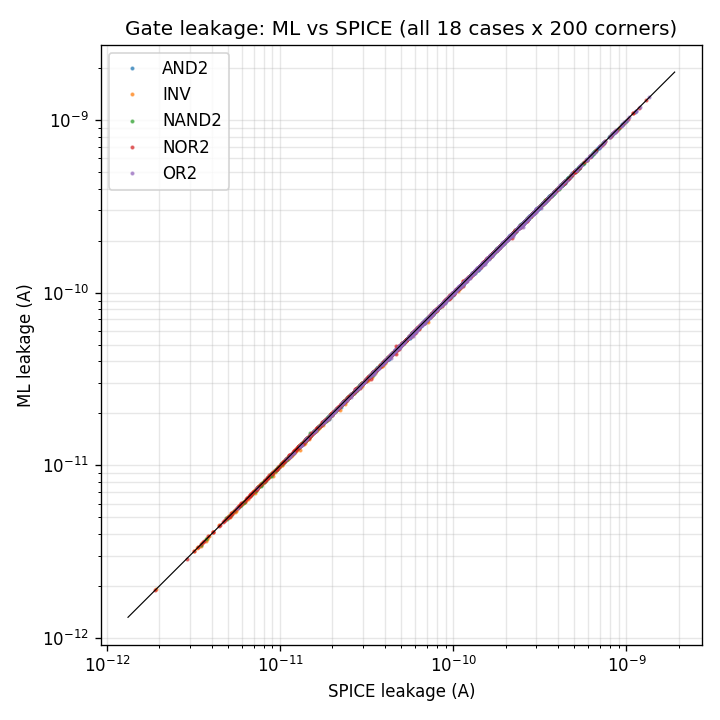
\includegraphics[width=.66\textwidth]{gate_parity.png}
\caption{ML versus SPICE leakage for all 3{,}600 gate simulations (18 cases $\times$ 200 corners), log axes; the line is $y=x$.}\label{fig:gparity}
\end{figure}

Over all 3{,}600 runs the \textbf{mean accuracy is 99.65\,\%}: median error 0.19\,\%, P95 1.2\,\%, largest error 5.7\,\%, bias $+0.03$\,\%.
Every one of the 18 cases reaches a mean accuracy of at least 99.4\,\%, and the leakage spans almost three decades
($2\times10^{-12}$ to $1.4\times10^{-9}$\,A) without visible deviation from the diagonal.
\begin{itemize}
  \item \textbf{Most accurate:} NAND2 (99.75\,\%), in particular NAND2\,00 and NAND2\,10 (median 0.09--0.11\,\%). Their leakage is dominated by gate
        tunnelling of ON PMOS devices with $V_d=V_s=\Vdd$, which the PMOS ON model predicts to within 0.1\,\%.
  \item \textbf{Least accurate:} INV\,0, INV\,1 and NOR2\,10 (mean accuracy 99.41--99.44\,\%). These are the cases in which a single OFF transistor
        carries a large share of the leakage---the OFF NMOS of INV\,0, the OFF PMOS of INV\,1 and the upper OFF PMOS ($W=4\Lmin$) of the NOR2 stack
        in NOR2\,10---so the error of the OFF channel-current model (1--3\,\%) is weighted more strongly than in the other gates
        (\cref{sec:errors}).
  \item AND2 and OR2 are about as accurate as NAND2 and NOR2 (99.66--99.70\,\%): the two stages are composed together and their errors partly average.
\end{itemize}
The internal node voltages used by the ML side are, by construction, those recorded by SPICE (step 1 above, as the assignment prescribes), so for every
run the internal node voltages of the SPICE and the ML evaluation are identical; both are stored with the run results
(\texttt{results/gates/gate\_runs\_ml.csv}, per-device inputs and predicted currents in \texttt{gate\_devices\_ml.csv}).

\section{Test-circuit validation: 8-bit parity checker}\label{sec:circuit}

\subsection{Circuit and SPICE reference}
The 8-bit parity checker outputs $1$ when an odd number of its eight inputs is $1$. No netlist is prescribed, so it was designed as a balanced tree of
seven XOR2 cells (four, two and one per level). Each XOR2 is the classic four-NAND2 realisation
\[
  n_1=\overline{a\,b},\qquad n_2=\overline{a\,n_1},\qquad n_3=\overline{b\,n_1},\qquad y=\overline{n_2\,n_3},
\]
so the circuit consists of 28 NAND2 gates (112 transistors, NAND2 sizing of \cref{sec:gates}) and every gate maps onto one of the four NAND2 input
cases of Part~B. The eight primary inputs are ideal sources at exactly $0$ or $\Vdd$ and the ground rail contains a 0\,V current probe, as in the
gate netlists (example netlists: \texttt{data/netlists/circuit/}).

The complete transistor-level netlist was simulated for all $2^8=256$ input vectors at the same 200 corners as the gates, i.e.\ $51{,}200$ SPICE runs,
each cross-checked as in \cref{sec:gates}. All runs converged with the mandated options, the cross-check agreed everywhere, and the output was at the
correct logic rail in every run, which confirms that the netlist implements the parity function.

\subsection{Hierarchical ML prediction}
For each input vector the logic value at the inputs of each of the 28 gates is found by logic propagation through the tree. The Part~B gate model of
that input combination, evaluated at the same corner, gives each gate's leakage, and the 28 gate leakages are summed
(\texttt{src/dvdml/circuit.py}, \texttt{scripts/09\_circuit\_ml.py}). As prescribed, this assumes that every gate input sits exactly at $0$ or $\Vdd$
and ignores loading between gates. The gate models in turn use only the four transistor models.

\subsection{Results}
\begin{table}[H]
\centering
{\small
\begin{adjustbox}{max width=\linewidth}
\begin{tabular}{lrrrrrrrr}
\toprule
input vectors & runs & SPICE median [A] & ML median [A] & bias & median err & P95 err & max err & mean acc. \\
\midrule
all 51,200 runs & 51200 & $2.87\times10^{-9}$ & $2.87\times10^{-9}$ & 0.14\% & 0.19\% & 0.79\% & 1.63\% & 99.73\% \\
0 ones in input & 200 & $3.33\times10^{-9}$ & $3.33\times10^{-9}$ & 0.14\% & 0.19\% & 0.74\% & 1.04\% & 99.75\% \\
1 ones in input & 1600 & $3.19\times10^{-9}$ & $3.19\times10^{-9}$ & 0.15\% & 0.19\% & 0.74\% & 1.09\% & 99.75\% \\
2 ones in input & 5600 & $3.10\times10^{-9}$ & $3.10\times10^{-9}$ & 0.14\% & 0.19\% & 0.76\% & 1.27\% & 99.74\% \\
3 ones in input & 11200 & $2.97\times10^{-9}$ & $2.97\times10^{-9}$ & 0.14\% & 0.19\% & 0.77\% & 1.29\% & 99.74\% \\
4 ones in input & 14000 & $2.90\times10^{-9}$ & $2.89\times10^{-9}$ & 0.14\% & 0.19\% & 0.79\% & 1.43\% & 99.73\% \\
5 ones in input & 11200 & $2.80\times10^{-9}$ & $2.80\times10^{-9}$ & 0.14\% & 0.19\% & 0.79\% & 1.45\% & 99.73\% \\
6 ones in input & 5600 & $2.74\times10^{-9}$ & $2.74\times10^{-9}$ & 0.13\% & 0.20\% & 0.80\% & 1.58\% & 99.72\% \\
7 ones in input & 1600 & $2.74\times10^{-9}$ & $2.74\times10^{-9}$ & 0.13\% & 0.20\% & 0.79\% & 1.55\% & 99.72\% \\
8 ones in input & 200 & $2.83\times10^{-9}$ & $2.84\times10^{-9}$ & 0.13\% & 0.20\% & 0.82\% & 1.63\% & 99.72\% \\
\bottomrule
\end{tabular}
\end{adjustbox}
}
\caption{Test-circuit results (8-bit parity checker, 256 input vectors $\times$ 200 corners): all runs, and grouped by the number of ones in the input vector.}
\label{tab:circuit}
\end{table}


\begin{table}[H]
\centering
{\small
\begin{adjustbox}{max width=\linewidth}
\begin{tabular}{lrrrrr}
\toprule
comparison & bias & median err & P95 err & max err & mean accuracy \\
\midrule
hierarchical ML vs circuit SPICE & 0.14\% & 0.19\% & 0.79\% & 1.63\% & 99.73\% \\
sum of isolated-gate SPICE vs circuit SPICE (loading only) & 0.00\% & 0.00\% & 0.01\% & 0.03\% & 100.00\% \\
\bottomrule
\end{tabular}
\end{adjustbox}
}
\caption{Source of the circuit-level error: ML prediction versus the error caused by ignoring loading between gates.}
\label{tab:cdecomp}
\end{table}



\begin{figure}[!htbp]\centering
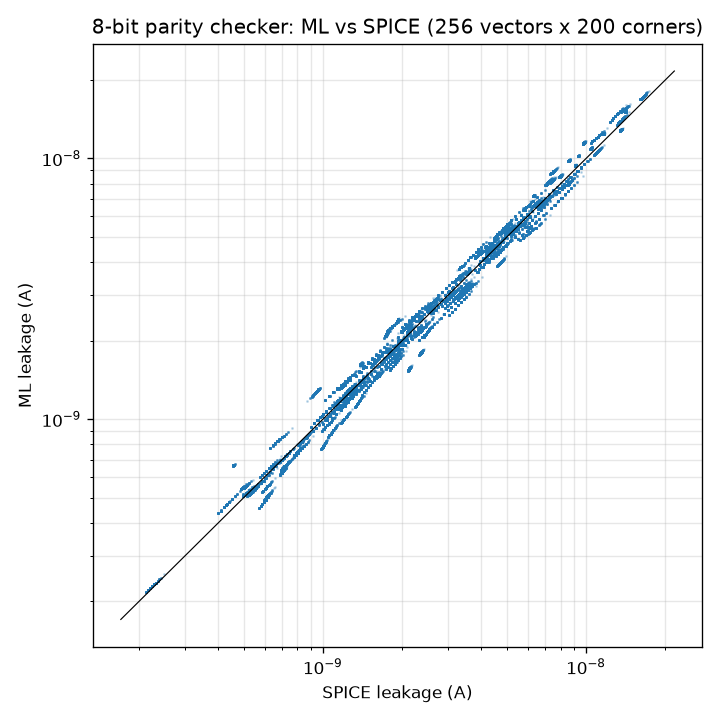
\includegraphics[width=.62\textwidth]{circuit_parity.png}
\caption{ML versus SPICE leakage of the 8-bit parity checker, all 51{,}200 runs (256 vectors $\times$ 200 corners), log axes.}\label{fig:cparity}
\end{figure}

Over all 51{,}200 runs the \textbf{mean accuracy is 99.73\,\%}: median error 0.19\,\%, P95 0.79\,\%, largest error 1.6\,\%, bias $+0.14$\,\%. The
accuracy does not depend on the input vector (99.72--99.75\,\% for zero to eight ones in the input).

\paragraph{Comparison with the gate level.} The assignment expects the circuit to be somewhat less accurate than the gates, because the composition
ignores loading. Here the circuit is as accurate as the gates (median 0.19\,\% at both levels), and its P95 and maximum errors are even lower
(0.79\,\% vs 1.2\,\%, 1.6\,\% vs 5.7\,\%). \Cref{tab:cdecomp} explains why: for rail-to-rail inputs, the sum of the SPICE leakages of the 28
\emph{isolated} gates reproduces the SPICE leakage of the complete circuit to within $10^{-4}$ (mean accuracy 99.996\,\%), so neglecting the loading
between gates costs essentially nothing and the circuit error is the error of the gate models. The circuit uses only NAND2 gates, which are the most
accurate gate type (\cref{tab:bygate}), and summing 28 gate leakages averages part of their random errors, which narrows the tails. The errors do not
average out completely, because all gates of one evaluation share the same corner and therefore the same systematic part of the model error
(\cref{sec:errors}).

\section{Error analysis}\label{sec:errors}
The run tables of \cref{sec:gates,sec:circuit} were grouped by corner condition (\texttt{scripts/10\_error\_analysis.py},
\texttt{results/error\_analysis/}). \Cref{fig:gcorner,fig:ccorner} show the error of every run against temperature, $\Vdd$ and the process draw.

\begin{figure}[!htbp]\centering
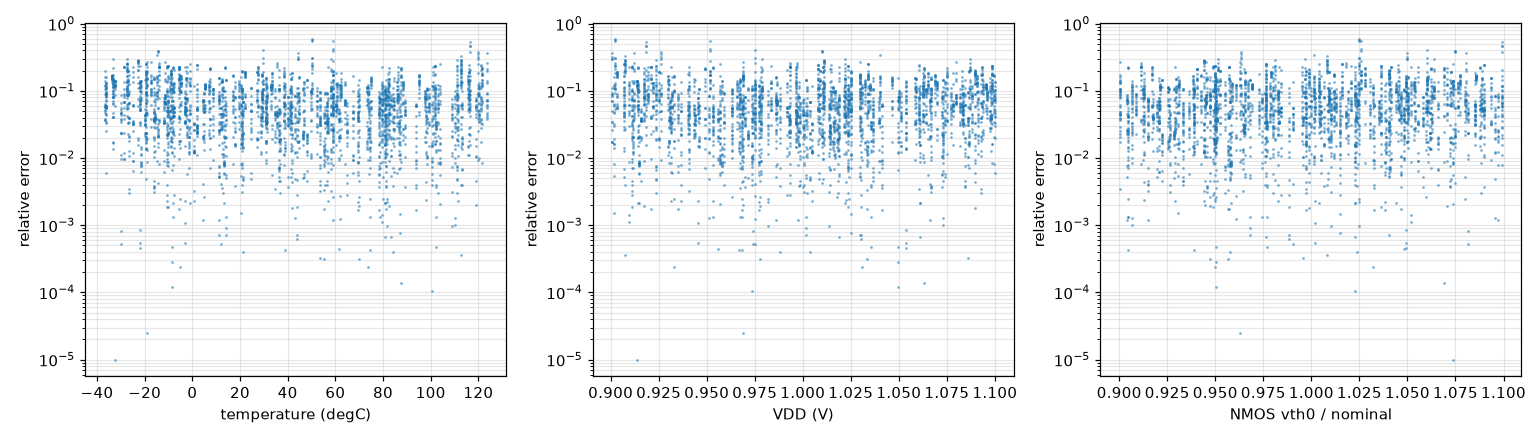
\includegraphics[width=\textwidth]{gate_error_vs_corner.png}
\caption{Gate level: relative error of all 3{,}600 runs against temperature, $\Vdd$ and the NMOS vth0 draw.}\label{fig:gcorner}
\end{figure}

\subsection{Where the largest errors occur}
\paragraph{High temperature.} The clearest dependence is on temperature (\cref{tab:gatecond}). Below $80\,^\circ$C the gate-level median error is
0.16--0.18\,\% and the P95 0.8--1.0\,\%; between $80$ and $125\,^\circ$C the median doubles to 0.33\,\%, the P95 rises to 2.2\,\%, the bias turns
negative ($-0.33$\,\%), and all of the ten largest errors occur above $100\,^\circ$C (\cref{tab:worst}).

\paragraph{Supply voltage.} The two ends of the $\Vdd$ range are slightly worse than the middle (P95 1.9\,\% and 1.3\,\% against 0.9--1.0\,\%), as
expected at the border of the sampled input range, where the networks have fewer neighbouring training points.

\paragraph{Process.} There is no systematic dependence on the vth0 draw: the median error is 0.16--0.20\,\% in every quarter of the NMOS and PMOS
vth0 range. A low threshold therefore matters only through the higher OFF current it causes (next paragraph), not by itself.
\begin{table}[H]
\centering
{\small
\begin{adjustbox}{max width=\linewidth}
\begin{tabular}{llrrrrr}
\toprule
condition & range & runs & bias & median err & P95 err & max err \\
\midrule
temperature [C] & -40 to 0 & 954 & 0.22\% & 0.16\% & 0.84\% & 2.89\% \\
temperature [C] & 0 to 40 & 846 & 0.16\% & 0.18\% & 0.76\% & 2.02\% \\
temperature [C] & 40 to 80 & 900 & 0.06\% & 0.17\% & 1.01\% & 3.26\% \\
temperature [C] & 80 to 125 & 900 & -0.33\% & 0.33\% & 2.24\% & 5.68\% \\
VDD [V] & 0.9 to 0.95 & 774 & -0.06\% & 0.25\% & 1.86\% & 5.68\% \\
VDD [V] & 0.95 to 1 & 936 & 0.06\% & 0.17\% & 0.98\% & 3.00\% \\
VDD [V] & 1 to 1.05 & 972 & 0.07\% & 0.16\% & 0.91\% & 4.66\% \\
VDD [V] & 1.05 to 1.1 & 918 & 0.03\% & 0.21\% & 1.25\% & 5.54\% \\
NMOS vth0 deviation & -10\% to -5\% & 936 & -0.01\% & 0.19\% & 1.25\% & 5.54\% \\
NMOS vth0 deviation & -5\% to +0\% & 918 & -0.01\% & 0.20\% & 1.50\% & 5.68\% \\
NMOS vth0 deviation & +0\% to +5\% & 1008 & 0.06\% & 0.17\% & 0.99\% & 5.07\% \\
NMOS vth0 deviation & +5\% to +10\% & 738 & 0.08\% & 0.20\% & 1.16\% & 3.26\% \\
PMOS vth0 deviation & -10\% to -5\% & 954 & -0.08\% & 0.20\% & 1.66\% & 4.75\% \\
PMOS vth0 deviation & -5\% to +0\% & 774 & 0.03\% & 0.16\% & 1.08\% & 5.07\% \\
PMOS vth0 deviation & +0\% to +5\% & 990 & 0.12\% & 0.20\% & 1.05\% & 5.54\% \\
PMOS vth0 deviation & +5\% to +10\% & 882 & 0.03\% & 0.20\% & 0.96\% & 5.68\% \\
\bottomrule
\end{tabular}
\end{adjustbox}
}
\caption{Gate-level (3{,}600 runs) error grouped by corner condition (vth0 deviation relative to the nominal value; negative = lower $|V_{th}|$).}
\label{tab:gatecond}
\end{table}


\begin{table}[H]
\centering
{\small
\begin{adjustbox}{max width=\linewidth}
\begin{tabular}{lrrrrrrrr}
\toprule
case & corner & VDD [V] & T [C] & NMOS vth0 [V] & PMOS vth0 [V] & SPICE [A] & ML [A] & error \\
\midrule
INV 0 & 45 & 0.9263 & 119.7 & 0.6634 & -0.6834 & $1.30\times10^{-11}$ & $1.22\times10^{-11}$ & -5.68\% \\
INV 0 & 168 & 1.073 & 110.1 & 0.6243 & -0.6481 & $7.16\times10^{-11}$ & $6.76\times10^{-11}$ & -5.54\% \\
INV 0 & 115 & 0.9074 & 112.8 & 0.6943 & -0.6089 & $9.08\times10^{-12}$ & $8.62\times10^{-12}$ & -5.07\% \\
NOR2 10 & 30 & 1.098 & 121.7 & 0.7078 & -0.6213 & $4.69\times10^{-11}$ & $4.92\times10^{-11}$ & 4.94\% \\
INV 0 & 54 & 1.098 & 101.6 & 0.6539 & -0.5767 & $3.40\times10^{-11}$ & $3.24\times10^{-11}$ & -4.75\% \\
NOR2 10 & 193 & 1.015 & 116.2 & 0.7198 & -0.5786 & $4.63\times10^{-11}$ & $4.41\times10^{-11}$ & -4.66\% \\
OR2 01 & 54 & 1.098 & 101.6 & 0.6539 & -0.5767 & $2.51\times10^{-10}$ & $2.40\times10^{-10}$ & -4.60\% \\
INV 0 & 83 & 1.062 & 120.2 & 0.6737 & -0.6936 & $2.20\times10^{-11}$ & $2.10\times10^{-11}$ & -4.59\% \\
NOR2 01 & 54 & 1.098 & 101.6 & 0.6539 & -0.5767 & $2.17\times10^{-10}$ & $2.07\times10^{-10}$ & -4.58\% \\
NOR2 00 & 45 & 0.9263 & 119.7 & 0.6634 & -0.6834 & $3.33\times10^{-11}$ & $3.18\times10^{-11}$ & -4.42\% \\
\bottomrule
\end{tabular}
\end{adjustbox}
}
\caption{The ten gate runs with the largest error and their corner conditions.}
\label{tab:worst}
\end{table}



\paragraph{Gates and input combinations.} INV\,0 accounts for five of the ten worst runs, followed by NOR2\,10 and the gates that contain an
inverter or a NOR2 stage with the same transistor states (OR2\,01, NOR2\,01, NOR2\,00).

\subsection{Why: the share of sub-threshold leakage}
For this low-power card the gate leakage at room temperature is almost entirely gate-oxide tunnelling of the ON transistors, which the ON models predict
to 0.1--0.6\,\%. Tunnelling depends only weakly on temperature, whereas the sub-threshold current of the OFF transistors grows by a factor of about
400 from $-40$ to $125\,^\circ$C (\cref{fig:trends}). \Cref{tab:offshare} quantifies this for the inverter, where exactly one transistor is OFF: the
OFF channel current carries 0.2\,\% (INV\,0) and 1.3\,\% (INV\,1) of the leakage below $0\,^\circ$C, but 13\,\% and 30\,\% above $80\,^\circ$C.
At hot corners the leakage is therefore increasingly set by the OFF channel-current models, whose errors (median 1--3\,\%, \cref{tab:chosen,tab:rails})
are an order of magnitude larger than those of the ON gate-current models. The error of the gate grows accordingly, from 0.09\,\% to 0.93\,\% median
for INV\,0. In addition, $125\,^\circ$C is the upper edge of the sampled temperature range, where the networks extrapolate least well, which explains
the small negative bias there. The same mechanism explains the least accurate gate cases (\cref{sec:gates}): INV\,0, INV\,1 and NOR2\,10 have a single
OFF device (the NOR2\,10 one is the wide $4\Lmin$ upper PMOS) carrying a large share of the leakage, whereas in NAND2\,00/10 the leakage is dominated
by ON-PMOS tunnelling and the error is 0.1\,\%.
\begin{table}[H]
\centering
{\small
\begin{adjustbox}{max width=\linewidth}
\begin{tabular}{llrrrr}
\toprule
case & T [C] & runs & OFF-channel share of leakage & median err & bias \\
\midrule
INV 0 & -40 to 0 & 53 & 0.16\% & 0.09\% & 0.04\% \\
INV 0 & 0 to 40 & 47 & 0.99\% & 0.13\% & -0.15\% \\
INV 0 & 40 to 80 & 50 & 4.56\% & 0.20\% & -0.41\% \\
INV 0 & 80 to 125 & 50 & 13.01\% & 0.93\% & -1.42\% \\
INV 1 & -40 to 0 & 53 & 1.26\% & 0.31\% & 0.45\% \\
INV 1 & 0 to 40 & 47 & 3.33\% & 0.34\% & 0.20\% \\
INV 1 & 40 to 80 & 50 & 14.47\% & 0.24\% & 0.03\% \\
INV 1 & 80 to 125 & 50 & 30.17\% & 0.66\% & -0.66\% \\
\bottomrule
\end{tabular}
\end{adjustbox}
}
\caption{Inverter: share of the leakage carried by the channel (sub-threshold) current of the OFF transistor, and the ML error, by temperature.}
\label{tab:offshare}
\end{table}



\subsection{Circuit level: corner-systematic error}
\begin{figure}[!htbp]\centering
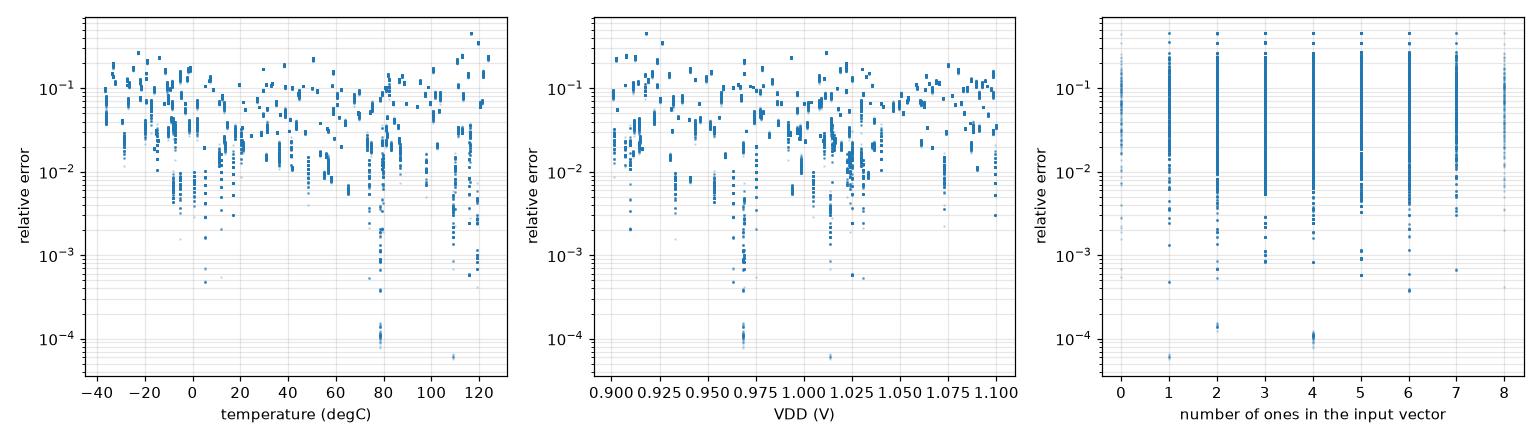
\includegraphics[width=\textwidth]{circuit_error_vs_corner.png}
\caption{Parity checker: relative error of all 51{,}200 runs against temperature, $\Vdd$ and the number of ones in the input vector.}\label{fig:ccorner}
\end{figure}
The circuit errors form vertical stripes in \cref{fig:ccorner}: at a given corner all 256 input vectors have almost the same error. The standard
deviation of the error between input vectors at one corner is only 0.011\,\%, while the mean error of a corner varies by 0.33\,\% (standard
deviation) between corners. All 28 gates of one evaluation share $\Vdd$, temperature and the process draw, so they share the systematic part of the
model error, which therefore does not average out over the circuit; only the random part does. The circuit inherits the temperature and $\Vdd$
dependence of the gates in weakened form (\cref{tab:circuitcond}): the median error is 0.25\,\% between $80$ and $125\,^\circ$C against 0.17--0.19\,\%
below, and the largest circuit error (1.6\,\%) occurs at the low end of the $\Vdd$ range.
\begin{table}[H]
\centering
{\small
\begin{adjustbox}{max width=\linewidth}
\begin{tabular}{llrrrrr}
\toprule
condition & range & runs & bias & median err & P95 err & max err \\
\midrule
temperature [C] & -40 to 0 & 13568 & 0.17\% & 0.19\% & 0.61\% & 0.80\% \\
temperature [C] & 0 to 40 & 12032 & 0.22\% & 0.18\% & 0.79\% & 0.85\% \\
temperature [C] & 40 to 80 & 12800 & 0.17\% & 0.17\% & 0.87\% & 1.63\% \\
temperature [C] & 80 to 125 & 12800 & -0.01\% & 0.25\% & 0.88\% & 1.35\% \\
VDD [V] & 0.9 to 0.95 & 11008 & 0.09\% & 0.23\% & 0.91\% & 1.63\% \\
VDD [V] & 0.95 to 1 & 13312 & 0.16\% & 0.18\% & 0.64\% & 1.05\% \\
VDD [V] & 1 to 1.05 & 13824 & 0.16\% & 0.18\% & 0.75\% & 1.01\% \\
VDD [V] & 1.05 to 1.1 & 13056 & 0.13\% & 0.25\% & 0.82\% & 0.88\% \\
NMOS vth0 deviation & -10\% to -5\% & 13312 & 0.14\% & 0.18\% & 0.74\% & 0.83\% \\
NMOS vth0 deviation & -5\% to +0\% & 13056 & 0.09\% & 0.17\% & 0.79\% & 1.07\% \\
NMOS vth0 deviation & +0\% to +5\% & 14336 & 0.17\% & 0.20\% & 0.75\% & 1.01\% \\
NMOS vth0 deviation & +5\% to +10\% & 10496 & 0.16\% & 0.28\% & 1.04\% & 1.63\% \\
PMOS vth0 deviation & -10\% to -5\% & 13568 & -0.02\% & 0.19\% & 0.87\% & 1.63\% \\
PMOS vth0 deviation & -5\% to +0\% & 11008 & 0.11\% & 0.13\% & 0.58\% & 0.79\% \\
PMOS vth0 deviation & +0\% to +5\% & 14080 & 0.28\% & 0.25\% & 0.86\% & 1.05\% \\
PMOS vth0 deviation & +5\% to +10\% & 12544 & 0.19\% & 0.21\% & 0.63\% & 0.82\% \\
\bottomrule
\end{tabular}
\end{adjustbox}
}
\caption{Parity-checker (51{,}200 runs) error grouped by corner condition (vth0 deviation relative to the nominal value; negative = lower $|V_{th}|$).}
\label{tab:circuitcond}
\end{table}



\subsection{Transistor level}
At transistor level the largest relative errors occur for the ON-state drain and source currents at small $V_{ds}$, where the channel current
passes through zero and changes sign (\cref{tab:chosen}). These currents do not enter the leakage (\cref{sec:gates_method}). The gate current of the
OFF devices lies entirely below the $10^{-15}$\,A numerical floor of the reference and cannot be learned or scored; its contribution to the leakage is
correspondingly negligible.

\subsection{Reference quality}
With the mandated tolerances alone, 3.5\,\% of the gate SPICE runs were invalid or did not converge (\cref{tab:ref}). Without the cross-check, these
runs would have appeared as ML errors of up to 100\,\%, although they are errors of the reference.

\section{Limitations and improvements}\label{sec:limits}
\todo{Final phase. Items already known: (i) numerical noise floor of the reference currents at about $10^{-15}$\,A; (ii) PD/PS junction perimeters not set;
(iii) gate leakage definition and gate sizing are assumptions pending TA confirmation; (iv) transistor models trained on a fixed oxide/process distribution only.}

\section{Conclusion}\label{sec:conclusion}
Machine-learning models trained only on single-transistor SPICE data of the assigned PTM 22\,nm LP card predict the leakage of CMOS gates and of an
8-bit parity checker under PVT variation with SPICE-level accuracy:
\begin{table}[H]
\centering
{\small
\begin{adjustbox}{max width=\linewidth}
\begin{tabular}{lrrrrrr}
\toprule
level & runs & bias & median err & P95 err & max err & mean accuracy \\
\midrule
gates (18 cases) & 3600 & 0.03\% & 0.19\% & 1.20\% & 5.68\% & 99.65\% \\
parity checker & 51200 & 0.14\% & 0.19\% & 0.79\% & 1.63\% & 99.73\% \\
\bottomrule
\end{tabular}
\end{adjustbox}
}
\caption{Headline accuracy of the ML leakage estimate against SPICE.}
\label{tab:headline}
\end{table}


\begin{itemize}
  \item Of four model types compared on the validation sets, the MLP was the most accurate for every transistor case. Specialising it per terminal
        current, with effective-width-normalised targets and training data at the rail corners where gates operate, raised the gate-level mean accuracy
        from 92.8\,\% to 99.65\,\%.
  \item A Kirchhoff-consistent composition of the transistor currents is essential: a plain sum of predicted terminal currents is off by orders of
        magnitude, because the channel current of the ON transistors in a leaking gate is set by the circuit, not by the device.
  \item The parity checker reaches 99.73\,\%: for rail-to-rail inputs, loading between gates is negligible, so the circuit inherits the gate accuracy.
  \item The remaining error is largest at hot corners, where sub-threshold leakage of the OFF transistors becomes significant, and it is shared by all
        gates of a corner.
\end{itemize}

\appendix
\section{Deliverables}\label{app:deliverables}
\begin{table}[H]
\centering
{\small
\begin{adjustbox}{max width=\linewidth}
\begin{tabular}{lllr}
\toprule
\# & deliverable & location & status \\
\midrule
1 & Datasets: 4 CSV files, 10,000 rows, 16 columns & data/transistor/ & present \\
2 & Example netlists: transistor (4), gates (18), test circuit & data/netlists/ & present \\
3 & Data check: Kirchhoff check and three trend plots & results/data\_check/ & present \\
4 & Model comparison table, 4 types x 4 cases (validation) & results/model\_comparison/ & present \\
5 & Chosen models: test errors, predicted-vs-SPICE plots, 4 model files & models/, results/models/ & present \\
6 & Gate results table (18 cases) & results/gates/gate\_results.csv & present \\
7 & Gate parity plot (log axes) & results/gates/gate\_parity.png & present \\
8 & Test-circuit results and parity plot & results/circuit/ & present \\
9 & Code: scripts run in order, fixed seeds & scripts/, src/dvdml/ & present \\
10 & Typed report & report/ & present \\
\bottomrule
\end{tabular}
\end{adjustbox}
}
\caption{Deliverables and their location in the repository (status checked automatically).}
\label{tab:deliv}
\end{table}



\section{Assumptions and open points}\label{app:assumptions}
The assignment leaves several points open; the choices made are listed here so that they can be corrected if the course staff decide otherwise.
\begin{enumerate}[nosep]
  \item \textbf{Junction geometry.} $AD=AS=W\cdot L_{diff}$, $L_{diff}=44\,\mathrm{nm}$ (course-group clarification); PD/PS not set. Adding PD$=$PS$=W+2L_{diff}$ changed only $I_b$, by about 10\,\% at the $10^{-12}$\,A level (one test point).
  \item \textbf{Noise floor.} Currents below $10^{-15}$\,A are numerical noise of the reference simulator; accuracy is reported on currents above this floor, together with the fraction of samples below it.
  \item \textbf{Gate leakage definition} (total current delivered by all sources at $V_{DD}$), \textbf{gate transistor sizing}, and \textbf{source of internal-node voltages in the circuit-level prediction}: see \texttt{docs/PROJECT\_CONTEXT.md}, questions Q1, Q2, Q6.
  \item \textbf{Accuracy definition.} Relative error $|I_{ML}-I_{SPICE}|/|I_{SPICE}|$; median and 95th percentile; bias is the mean signed relative error.
\end{enumerate}
\todo{Update after TA answers.}

\section{Reproducing the results}\label{app:reproduce}
Requirements: \href{https://docs.astral.sh/uv/}{uv} (installs Python 3.12 and the locked package versions) and ngspice-47 (\texttt{NGSPICE\_EXE}
pointing to the console executable). From the repository root:
{\scriptsize
\begin{verbatim}
uv sync                                                  # .venv with the versions in uv.lock
uv run python scripts/00_check_env.py                    # package and ngspice versions
uv run python scripts/01_generate_transistor_data.py     # 4 x 10,000 rows + example netlists     (SPICE)
uv run python scripts/01b_generate_extra_data.py         # 4 x 30,000 extra uniform rows           (SPICE)
uv run python scripts/01c_generate_edge_data.py          # 4 x 20,000 rail-corner rows             (SPICE)
uv run python scripts/02_data_check.py                   # Kirchhoff check, distributions, trends  (SPICE)
uv run python scripts/03_make_splits.py                  # 70/15/15 split, fixed seed
uv run python scripts/04_compare_models.py               # 4 model types x 4 cases on validation
# final per-current models: seven training runs (exact commands in README.md)
uv run python scripts/05d_train_per_current.py ...       # GPU optional: --device cuda | cpu
uv run python scripts/05e_evaluate_v2.py                 # test-set metrics, predicted-vs-SPICE plots
uv run python scripts/06_gate_spice.py                   # 200 corners x 18 gate cases             (SPICE)
uv run python scripts/07_gate_ml.py                      # gate-level ML vs SPICE
uv run python scripts/08_circuit_spice.py                # parity checker, 51,200 runs             (SPICE)
uv run python scripts/09_circuit_ml.py                   # circuit-level ML vs SPICE
uv run python scripts/10_error_analysis.py               # error by corner condition
uv run python scripts/11_build_report_tables.py          # report/tables/*.tex
cd report && latexmk -pdf report.tex
\end{verbatim}}
All random draws use fixed seeds from \texttt{config/project.yaml}. Scripts 05e, 07, 09, 10 and 11 need only the committed data and models
(no SPICE, no training) and run in about a minute; they reproduce the committed results to within $10^{-10}$ (checked on Windows and macOS).
The SPICE steps take about 2--5 minutes per transistor dataset, under a minute for the gates and about 30 minutes for the parity checker; training all
16 networks takes about 2.5 hours on a laptop GPU.


\end{document}
